%%%%%%%%%%%%%%%%%%%%%%%%%%%%%%%%%%%%%%%%%%%%%%%%%%%%%%%%%%%%%%%%%%%%%%%%%%%%%%%%
\section{Cosine of Surface Orientations}\label{sec:singl_img_cosine_orientations}
%%%%%%%%%%%%%%%%%%%%%%%%%%%%%%%%%%%%%%%%%%%%%%%%%%%%%%%%%%%%%%%%%%%%%%%%%%%%%%%%
In this section we describe the theory behind building robust dissimilarity
measures by utilising the cosine function. We consider a
dissimilarity measure to be robust if it suppresses the contribution of
comparisons between image areas that are unrelated. More specifically, we seek a
measure that, when given two images that are visually dissimilar, will calculate
zero correlation between them. Suppressing the contribution of outliers is
a well studied area of mathematics and one flexible method of achieving this
is to employ a weighted comparison. A weighted comparison can be constructed
such that image areas that contain outliers are given a zero weighting and thus
do not bias the comparison between images in regions excluding the outlier.
This is useful for applications such as facial image alignment whereby an image
may contain gross outliers in the form of occlusions such as ``hand over the
face'' gestures. In this scenario, it is still appropriate to attempt to
align a facial model to the occluded input image and seek to suppress
the effect of the region of the face where the hand appears. This is also
appropriate in the case of statistical SfS which may also contain outliers
such as shadows and gesture occlusions. Unfortunately, identifying the outlier
regions is a challenging problem that likely requires complex scene
understanding in order to achieve accurately.
To this end, \citet{tzimiropoulos2012subspace} proposed the use of the cosine
function to provide a non-parametric method for suppressing outliers which
is shown to be equivalent to an automatically weighted dissimilarity measure.
Given the periodic domain of the cosine function is it desirable for the
input to also be bounded in a similar periodic range. For this reason,
\citet{tzimiropoulos2012subspace} propose to use polar coordinates to encode
the orientation of the normalised gradient, which is naturally bounded in the
$[0, 2\pi)$ range. This was utilized for both facial
alignment~\cite{tzimiropoulos2011robust,tzimiropoulos2014active,%
antonakos2015feature} and component
analysis~\cite{tzimiropoulos2012subspace,tzimiropoulos2014active}.

We propose to utilise the cosine function to construct robust dissimilarity
measures for surface normals. Given that surface normals also encode a local
measure of surface orientation they are well suited as inputs to the cosine
function. It is necessary, however, to make a clear distinction as to the
dimensionality of the data being considered. For the original work
on the cosine of normalised image gradients~\cite{tzimiropoulos2012subspace}
the input data were 2D images. In this work, we consider two forms of three
dimensional data: \textbf{2.5D data} and \textbf{3D or volumetric data}.
2.5D data is commonly represented in the form of surfaces and we define
the surface normal to be the unit vector perpendicular to the plane
tangent to a point on the surface. This surface normal contains
two degrees of freedom and is assumed to be a unit vector. 3D or volumetric
data is the direct extension of 2D images into the true third dimension
whereby the discrete elements composing the image are 3D voxels as opposed to
2D pixels. In this case, a true third dimension exists and gradients (which
are analogous to normals) are defined in a manner similar to 2D gradients. This
form of data is very common in the medical imaging community, for example.
We also note that the cosine \textit{dissimilarity measure} is defined as being
\textit{minimised} when the image areas are identical (minimum error is 0).
Conversely, the cosine \textit{similarity measure} is \textit{maximised} when
the image  areas are identical (maximum error is 1). Therefore, the
cosine measure is naturally defined as a similarity measure since when
two angles are identical their difference is 0 and thus $\cos(0) = 1$. The
cosine dissimilarity is trivially defined as $1 - \cos(\cdot)$ due to the range
of the cosine, $[-1, 1]$.

The remainder of this section will explain the assumptions and theory around
utilising the cosine function as a robust dissimilarity measure. We then
provide uses of the measure in the form of parametric SfS, 2.5D face
alignment using depth data and volumetric 3D image alignment.
%%%%%%%%%%%%%%%%%%%%%%%%%%%%%%%%%%%%%%%%%%%%%%%%%%%%%%%%%%%%%%%%%%%%%%%%%%%%%%%%
\subsection{Cosine Similarity in 2D}\label{subsec:singl_img_cosine_2d}
%%%%%%%%%%%%%%%%%%%%%%%%%%%%%%%%%%%%%%%%%%%%%%%%%%%%%%%%%%%%%%%%%%%%%%%%%%%%%%%%
Assuming we are given two 2D images, denoted as $I_i, \; i \in \{1,2\}$, we
define $G_{i,x} = \bb{F}_x \ast I_i$ and $G_{i,y} = \bb{F}_y \ast I_i$
as the gradients obtained by convolving $I_i$ with differentiation approximation
filters $\bb{F}_x$ and $\bb{F}_y$ respectively. We denote the
lexicographical vectorisation of $G_{i,x}$ as $\bb{g}_{i,x}$ and define an
index $k$ into the vector, $\bb{g}_{i,x}(k)$. We define an identical vector
for $G_{i,y}$ as $\bb{g}_{i,y}$. We also define $\bb{g}_{i}(k)$ as the
vector formed by concatenating the $x$ and $y$ gradients together. Trivially, we
can define the normalised gradient as
$\bb{\tilde{g}}_{i}(k) = \frac{\bb{g}_{i}(k)}{\norm{\bb{g}_{i}(k)}}$ where
$\norm{\bb{g}_{i}(k)} = \sqrt{{g_{i,x}(k)}^2 + {g_{i,y}(k)}^2}$.  We also define
similar vectors for the $x$ and $y$ components separately, with
$\bb{\tilde{g}}_{i,x}$ being the $x$ components concatenated in
lexicographical ordering and $\bb{\tilde{g}}_{i,y}$ being the $y$ components.
Finally, $\bb{\tilde{g}}_{i}$ is the vector of concatenated normalised
gradients for image $I_i$.

Given the normalised gradients, it is simple to parametrise them within a polar
coordinate system with radius $r_i(k) = \lVert \bb{\tilde{g}}_{i}(k) \rVert = 1$,
orientation $\phi_i(k) = \arctan{\frac{\tilde{g}_{i,y}(k)}{\tilde{g}_{i,x}(k)}}$
and pole at the origin.
Given orientations from two dissimilar images, it is reasonable to assume that
difference between the orientations, $\Delta \phi(k) = \phi_1(k) - \phi_2(k)$,
can take any angle between $[0, 2\pi)$. Intuitively, this implies that selecting
two pixels from dissimilar images is unlikely to yield any correlation between
the images.
In~\cite{tzimiropoulos2011robust,tzimiropoulos2012subspace},
it was experimentally verified that the
orientation differences follow a uniform distribution, $\Delta \phi(k) \sim U(0,
2\pi)$. The fact that the orientation differences follows a uniform distribution
is unsurprising under the assumption that the two images have absolutely no
correlation. However, the expectation of the cosine of the uniform distribution
is zero, which is a powerful property that can be exploited for image
registration. It is powerful because it means that the expected overall
contribution of uncorrelated areas to any cost function will be zero, meaning
the uncorrelated areas do not affect the result of the registration.

Formally, we assume $\Delta \phi(k)$ is a stationary random process $y(t)$ with
index $t \triangleq k \in \mathcal{R}^2$, where $\forall t \sim U(0, 2\pi)$. We
define the random process $z(t) = \cos{y(t)}$ and thus $\forall t$ random
variable $Z = z(t)$ has mean value $E\{Z\} = 0$. In fact, by assuming mean
ergodicity, we find that
%%%%%%%%%%%%%%%%%%%%%%%%%%%%%%%%%%%%%%%%%%%%%%%%%%%%%%%%%%%%%%%%%%%%%%%%%
\begin{equation}\label{eq:cosine_integral}
    E\{Z\} \propto \int z(t) dt \equiv \int_{\mathcal{R}^2} \cos[\Delta \phi(k)] \; dk = 0
\end{equation}
%%%%%%%%%%%%%%%%%%%%%%%%%%%%%%%%%%%%%%%%%%%%%%%%%%%%%%%%%%%%%%%%%%%%%%%%%
This is an important property for a similarity measure to be robust against
occlusions. Since occlusions do not provide useful information for alignment,
ideally they would be ignored. However, manual segmentation of occluded areas is
time consuming and prone to error. Therefore, an ideal robust similarity measure
would be able to automatically identify regions of the image that are occluding
the true object of interest. Under the previous definition of robustness, the
cosine similarity naturally represents a robust similarity measure as it
automatically suppresses the contribution of outliers.

In practise, when comparing two images where one image contains occlusions,
there will be regions that are correlated and then the occluded region that is
uncorrelated. In this case, the total distribution of all pixels will be
described by a mixture model of the occluded and non-occluded regions. We desire
that the distribution of the uncorrelated areas has an expectation of zero and
thus will not affect the optimisation of the similarity measure.
%%%%%%%%%%%%%%%%%%%%%%%%%%%%%%%%%%%%%%%%%%%%%%%%%%%%%%%%%%%%%%%%%%%%%%%%%%%%%%%%
\subsection{Cosine Similarity in 2.5D and 3D}\label{subsec:singl_img_cosine_3d}
%%%%%%%%%%%%%%%%%%%%%%%%%%%%%%%%%%%%%%%%%%%%%%%%%%%%%%%%%%%%%%%%%%%%%%%%%%%%%%%%
Measuring the angular distance between vectors in three dimensional spaces
is more complex than in 2D, due to the extra degree of freedom. In the following
section, we describe two different measures that can be used to calculate
similarities between vectors within 3D spaces, the spherical coordinates and the
inner product. In the previous section, we described in detail how properties of
the cosine of a uniform distribution can be exploited to form a robust measure
of similarity. The most important property was that uncorrelated areas such as
occlusions should have no impact on similarity measurement. This was formalised
as the fact that the expectation of the sum of the uncorrelated elements should
be zero. In the case of input to the cosine function, a given distribution must
simply be symmetric over the positive and negative span of outputs of the
cosine. When symmetric over the positive and negative outputs, the expectation
of the cosine function is zero. In fact, we can relax the definition of a
measure being robust to outliers by stating that we actually desire a measure
whereby the \textit{expectation of the measure over image areas that are
uncorrelated is zero}.

In this section we consider two forms of three dimensional
data: 2.5D and volumetric 3D. \textbf{2.5D data} is defined as a surface composed
of a set of 3D coordinates, typically related by triangulation such that
the surface is composed of a set of triangular facets. In contrast to 3D data,
these 2.5D points are not a discretisation of the 3D space and thus there
is no concept of a voxel. Typically, 2.5D data is produced via a projection
of the 3D world with respect to a viewing plane. For example, depth data, as
recovered from systems such as the Microsoft Kinect~\cite{zhang2012microsoft}
represents 2.5D data with respect to the Kinect sensor plane. Although any
arbitrary mesh would be considered 2.5D under this definition, in this work
we consider 2.5D data recovered from imaging devices such as the Kinect and thus
there is an implicit connectivity between neighbouring points. This connectivity
is a regular lattice in the $x-y$ plane that is analogous with pixels and thus
the data can be thought of as a depth or height map. Therefore, image indexing
returns the appropriate depth/height for a given projected pixel.

The spherical coordinate system and the dot product are applicable for
both 2.5D data and 3D/volumetric data. In the case of 2.5D data, the spherical
coordinates are derived from the vector perpendicular to the plane tangent
to any point on the 2.5D surface. For example, given a 2.5D surface parametrised
by a set of triangular facets, the surface normal for a given triangle
can be found by computing a cross product between two of the triangles edges.
Assuming depth data, as mentioned previously, each pixel is analogous to a single
depth value and thus the sampled normal for a depth value corresponds to a
vertex normal. A vertex normal is simply computed by averaging the normals
corresponding to the centre of each triangular facet that a given vertex is
a part of.

Formally, assuming we are given two 2.5D images,
denoted as $D_i, \; i \in \{1,2\}$, we define $\bb{d}_i$ as the lexicographical
vectorisation of $D_i$ which can be indexed by the linear index $k$ as
$\bb{d}_i(k)$. We also assume triangulation matrices
$\bb{T}^i \in \R^{m \times 3}$ where $m$ is the number of triangles and each row
provides the set of linear indices into $\bb{d}_i$ that index the vertices
that compose a triangle. The per triangle normal for row $q$ can be computed as
${\bb{T}^i}_{q\ast} = [a_q, b_q, c_q]$ and
$\bb{\hat{n}}^q = ({\bb{d}_i(b_q)} - {\bb{d}_i(a_q)}) \times ({\bb{d}_i(c_q)} - {\bb{d}_i(a_q)})$
where $\times$ denotes the vector cross product. To represent a valid normal,
$\bb{\hat{n}}^q$ must be normalised to a unit vector,
$\bb{n}^q = \frac{\bb{\hat{n}}^q}{\norm{\bb{\hat{n}}^q}}$. The per vertex normal
is computed as the average of all the per triangle normals that a vertex
is a part of. Therefore, the corresponding vertex normal for index $k$ into
$\bb{d}_i(k)$ is defined as $\bb{\hat{n}}_{i,k} = \frac{1}{t} \sum_{q \in Q} \bb{n}^q$
where $Q \in \R^t$ is the set of indices of the triangles that the vertex at index
$k$ is a part of. Note that $\bb{\hat{n}}_{i,k}$ must also be normalised to
a unit vector $\bb{n}_{i,k} = \frac{\bb{\hat{n}}_{i,k}}{\norm{\bb{\hat{n}}_{i,k}}}$.
It should also be noted that for the case of 2.5D images that are triangulated
over a regular grid, the normals can also be computed using the
identity given by \cref{eq:bg_sfs_normal_pq} in a manner similar to the 2D
gradient procedure described above.
Note that the direction of the  normal with respect to which ``side'' of the
surface it extends from, \eg~the sign of the normal, is unimportant and need
only be consistent between all computed normals. In this work, we assume that
normals always point ``outward'' towards the camera and away from the surface
centre of mass.

For 3D images, we make very similar
assumptions to those made in \cref{subsec:singl_img_cosine_2d} for 2D images.
We simply extend the notation of \cref{subsec:singl_img_cosine_2d} by including the
gradient of the $z$-axis, denoted as $G_{i,z} = \bb{F}_z \ast I_i$.
We also redefine the normalised gradient as
$\bb{\tilde{g}}_{i}(k) = \frac{\bb{g}_{i}(k)}{\norm{\bb{g}_{i}(k)}}$
where $\norm{\bb{g}_{i}(k)} = \sqrt{{g_{i,x}(k)}^2 + {g_{i,y}(k)}^2 +
{g_{i,z}(k)}^2}$ and $\bb{g}_{i}(k)$ is defined as the vector formed by
concatenating the $x$, $y$ and $z$ gradients together. Although the
computation of spherical coordinates and the inner product are identical for
both surface normals and 3D gradients, we disambiguate between the two and
always denote surface normals with $\bb{n}$ and 3D gradients with $\bb{g}$.
%%%%%%%%%%%%%%%%%%%%%%%%%%%%%%%%%%%%%%%%
\begin{figure}
    \centering
    \begin{subfigure}{0.32\textwidth}
        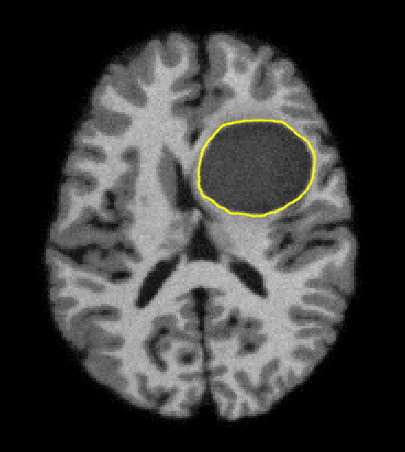
\includegraphics[width=\textwidth]{statistical_normals/images/tumour_example_axial}
    \end{subfigure}
    \begin{subfigure}{0.32\textwidth}
        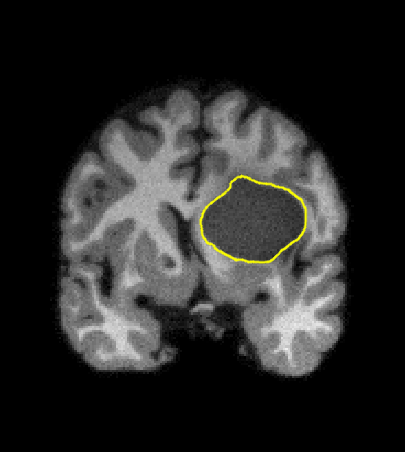
\includegraphics[width=\textwidth]{statistical_normals/images/tumour_example_coronal}
    \end{subfigure}
    \begin{subfigure}{0.32\columnwidth}
        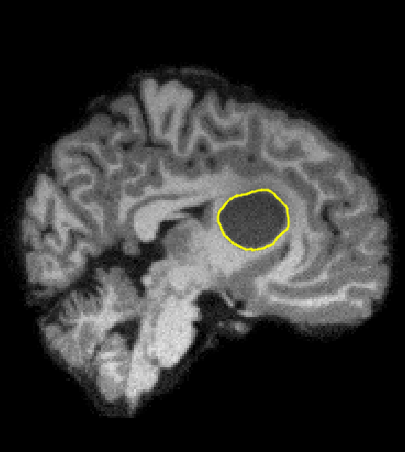
\includegraphics[width=\textwidth]{statistical_normals/images/tumour_example_sagital}
    \end{subfigure}
    \caption{Example images of a T1-weighted brain containing a tumour area. 
             The tumour areas are outlined in yellow in each image.
             Left: Axial View. Middle: Coronal View. Right: Sagital View.}
\label{fig:singl_img_tumour_examples}
\end{figure}
%%%%%%%%%%%%%%%%%%%%%%%%%%%%%%%%%%%%%%%%

In \cref{subsubsec:singl_img_cosine_spherical} and
\cref{subsubsec:singl_img_cosine_inner_product} we describe two measures of angular
difference between 3D orientations. We investigate the distribution of these
angular measures when combined with the cosine function and motivate that they
are both suitable for use as a similarity measure between real data.
Unfortunately, whilst both the spherical coordinates and inner product kernels
can be computed for a 2.5D image,
there does not exist a gradient in the third dimension (z-dimension) and thus
much of the mathematical analysis on the robustness of the 2.5D features does 
not directly apply. However, in 
\cref{subsec:singl_img_lk_2d} we show that although the more rigorous technical
analysis of the robustness of the kernel spaces do not necessarily
hold in 2.5D, the kernels can still be used to construct
powerful feature descriptors. Therefore, for the rest of the section we consider
only the case of 3D/volumetric images.
%%%%%%%%%%%%%%%%%%%%%%%%%%%%%%%%%%%%%%%%%%%%%%%%%%%%%%%%%%%%%%%%%%%%%%%%%%%%%%%%
\subsubsection{Spherical Coordinates}\label{subsubsec:singl_img_cosine_spherical}
%%%%%%%%%%%%%%%%%%%%%%%%%%%%%%%%%%%%%%%%%%%%%%%%%%%%%%%%%%%%%%%%%%%%%%%%%%%%%%%%
%%%%%%%%%%%%%%%%%%%%%%%%%%%%%%%%%%%%%%%
\begin{figure}
    \centering
    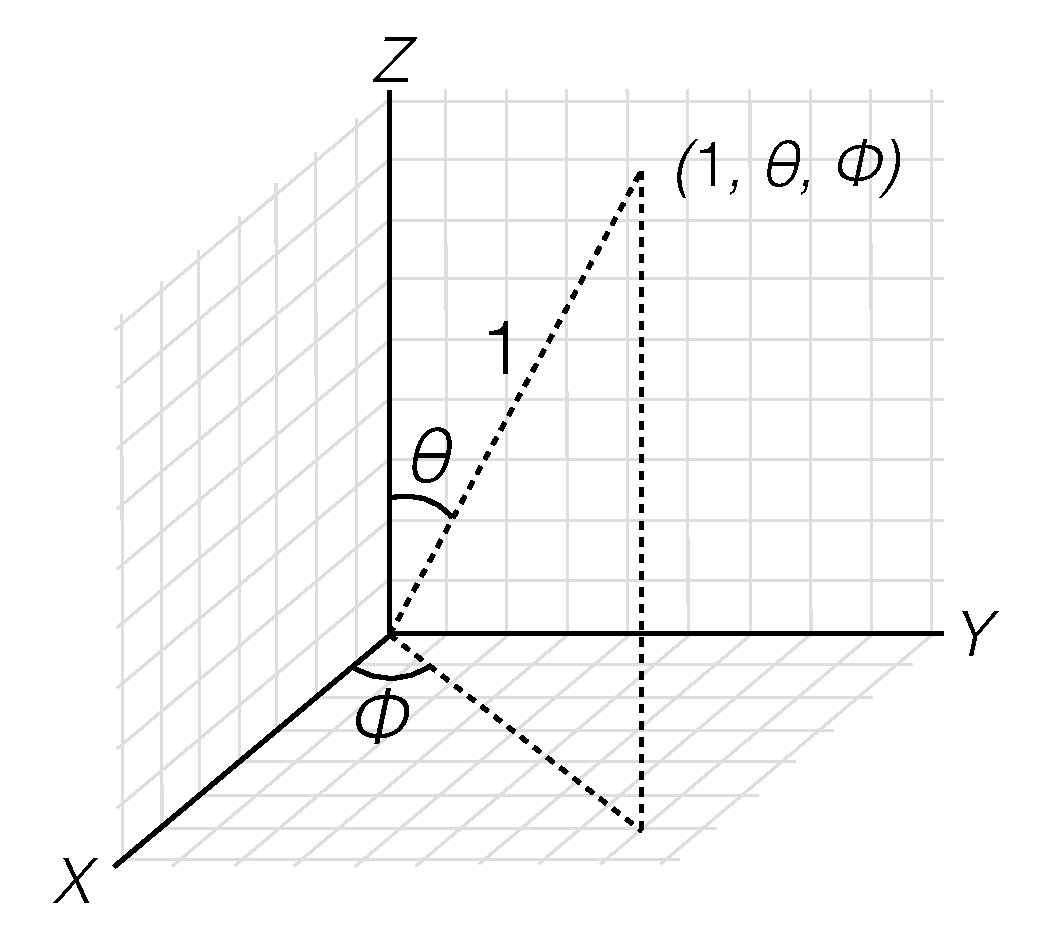
\includegraphics[width=0.5\textwidth]{statistical_normals/images/spherical_coords_example}
    \caption{An illustration of the spherical coordinate system assumed in this
             work. $\theta \in [0, \pi]$ defines the elevation angle and
             $\phi \in [0, 2\pi]$ defines the azimuth angle.}
\label{fig:singl_img_spherical_coords_example}
\end{figure}
%%%%%%%%%%%%%%%%%%%%%%%%%%%%%%%%%%%%%%%
In 2D, a natural parametrisation of the angle between the two gradient vectors
is the polar coordinate system. In 3D, we have three gradient vectors and thus
require two angles to describe their orientation. Unlike in 2D, where the
vectors lie on the unit circle, in 3D the vectors lie on the surface of a unit
sphere. Therefore, it is possible to parametrise the vectors in terms of the
spherical coordinate system, which is described by two angles: the azimuth angle
$\phi$ with range $[0, 2\pi)$ and the elevation angle $\theta$ with range
$[0, \pi]$. Denoting ${\bb{\tilde{x}}_i}(k)$ as the $k$th normalised gradient
for the $i$th image, either volumetric or 2.5D, we can calculate the spherical angles as follows:
%%%%%%%%%%%%%%%%%%%%%%%%%%%%%%%%%%%%%%%%%%%%%%%%%%%%%%%%%%%%%%%%%%%%%%%%%
\begin{equation}\label{eq:cartesian_to_spherical}
    \begin{aligned}
        r_i(k)      &= \lVert \bb{\tilde{x}}_{i}(k) \rVert = 1            \\
        \phi_i(k)   &= \arctan{\frac{\tilde{x}_{i,y}(k)}{\tilde{x}_{i,x}(k)}} \\
        \theta_i(k) &= \arccos{\tilde{x}_{i,z}(k)}
    \end{aligned}
\end{equation}
%%%%%%%%%%%%%%%%%%%%%%%%%%%%%%%%%%%%%%%%%%%%%%%%%%%%%%%%%%%%%%%%%%%%%%%%%
An illustration of the spherical coordinate system, as used in this paper, is
given in \cref{fig:singl_img_spherical_coords_example}.

Our proposal is to combine the spherical coordinates with the cosine function in
order to provide a robust similarity measure. Similar to the 2D case, we
propose the cosine of azimuth differences, $\Delta \phi = \phi_1 - \phi_2$, and
the cosine of elevation differences, $\Delta \theta = \theta_1 - \theta_2$, as a
combined similarity measures. Given a 3D image warping function with parameters
$\bb{p}$, the spherical coordinates form a similarity measure as follows:
%%%%%%%%%%%%%%%%%%%%%%%%%%%%%%%%%%%%%%%%%%%%%%%%%%%%%%%%%%%%%%%%%%%%%%%%%
\begin{equation}\label{eq:spherical_similarity_measure}
    q = \sum_k \cos \left(\Delta \phi(k)[\bb{p}]\right) + \sum_k \cos \left(\Delta \theta(k)[\bb{p}]\right)
\end{equation}
%%%%%%%%%%%%%%%%%%%%%%%%%%%%%%%%%%%%%%%%%%%%%%%%%%%%%%%%%%%%%%%%%%%%%%%%%
%%%%%%%%%%%%%%%%%%%%%%%%%%%%%%%%%%%%%%%%
\begin{figure}
    \centering
    \hspace*{\fill}
    \begin{subfigure}[b]{0.46\columnwidth}
    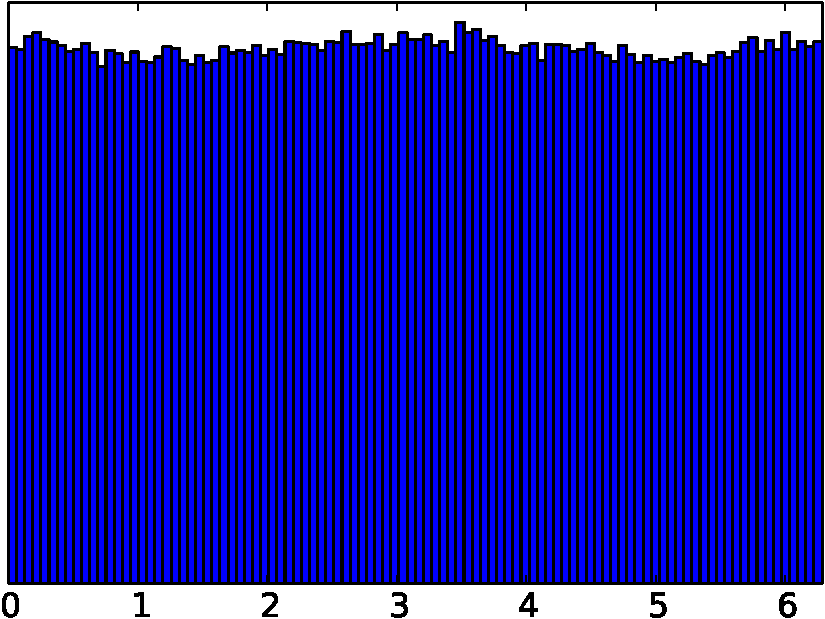
\includegraphics[width=\textwidth]{statistical_normals/images/distributions/delta_phi_tumour-crop}
    \caption{}\label{subfig:singl_img_phi_tumour}
    \end{subfigure}
    \hfill
    \begin{subfigure}[b]{0.45\columnwidth}
    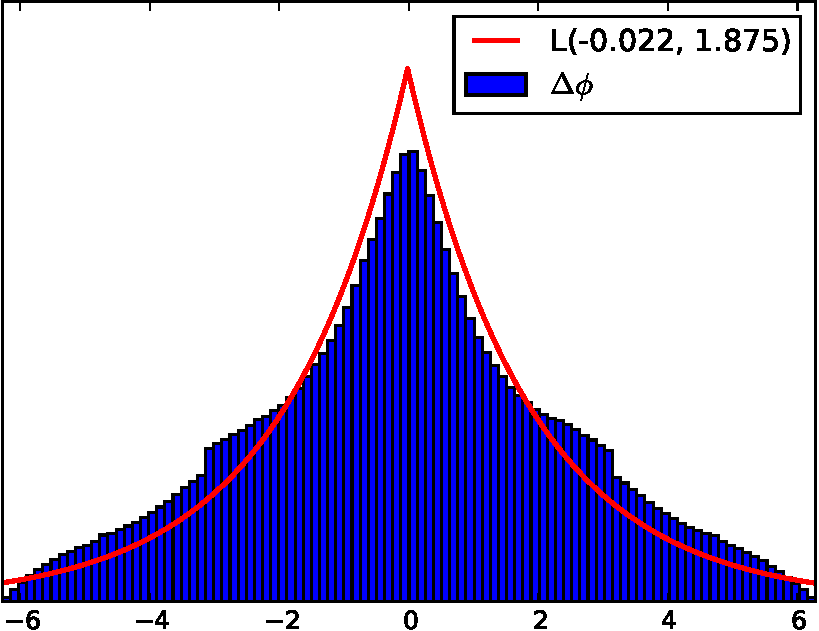
\includegraphics[width=\textwidth]{statistical_normals/images/distributions/delta_phi_all_laplacian-crop}
    \caption{}\label{subfig:singl_img_phi_all}
    \end{subfigure}
    \hspace*{\fill}
    \caption{The mean distribution of $\Delta \phi$ of the BraTS simulated images.
             The images were registered using a
             rigid transformation and only the tumour
             areas were sampled. (a) the distribution of $\Delta \phi$
             in the simulated tumour region. (b) the distribution of
             $\Delta \phi$ over the entire image. It also shows the
             Laplacian distribution that best fits the data.}
\label{fig:singl_img_phi_distribution}
\end{figure}
%%%%%%%%%%%%%%%%%%%%%%%%%%%%%%%%%%%%%%%%

Experimentally, we verified that $\Delta \phi$ approximates a symmetric
distribution for simulated tumour data taken from the Multimodal Brain Tumour
Image Segmentation (BraTS) challenge, as shown in
\cref{fig:singl_img_phi_distribution}. \cref{subfig:singl_img_phi_tumour} shows the
distribution of $\Delta \phi$ between the tumour area circled in yellow in
\cref{fig:singl_img_tumour_examples} and a healthy brain. The images were registered
using a rigid transformation before $\Delta \phi$ was computed.  The azimuth
angle is analogous to the angle studied in~\cite{tzimiropoulos2011robust} 
and follows the same uniform distribution, $\Delta \phi \sim U(0, 2\pi)$.

When the entire region of the rigidly registered brain images is considered, we
find that the distribution of $\Delta \phi$ is clearly a mixture of two separate
models, one for the occluded area and one for the rigidly registered area.
\cref{subfig:singl_img_phi_all} shows the distribution of $\Delta \phi$ calculated
over the entire image region of each image and a Laplacian distribution that
best fits the data. Thus, our experimental evidence suggests that the total
distribution of $\Delta \phi$ over the entire image region is a mixture model
between a uniform distribution and a Laplacian distribution with approximately
zero mean.
%%%%%%%%%%%%%%%%%%%%%%%%%%%%%%%%%%%%%%%%%%%%%%%%%%%%%%%%%%%%%%%%%%%%%%%%%%%%%%%%
\subsubsection{Inner Product}\label{subsubsec:singl_img_cosine_inner_product}
%%%%%%%%%%%%%%%%%%%%%%%%%%%%%%%%%%%%%%%%%%%%%%%%%%%%%%%%%%%%%%%%%%%%%%%%%%%%%%%%
%%%%%%%%%%%%%%%%%%%%%%%%%%%%%%%%%%%%%%%%
\begin{figure*}
    \centering
    \hspace*{\fill}
    \begin{subfigure}[t]{0.32\textwidth}
        \centering
        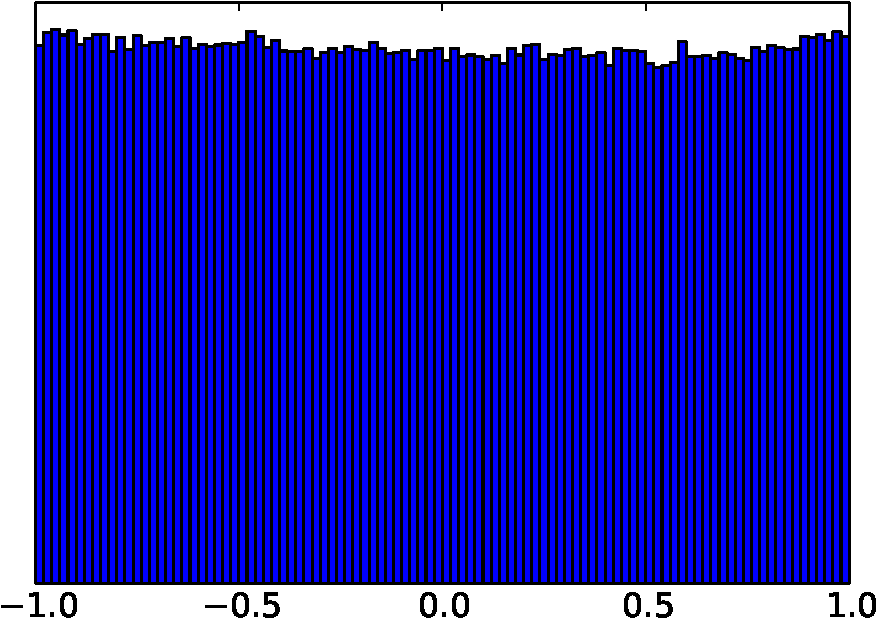
\includegraphics[width=\textwidth]{statistical_normals/images/distributions/inner_product_tumour-crop}
        \caption{$\cos{\sigma}$ tumour area}\label{subfig:singl_img_inner_product_tumour}
    \end{subfigure} \hfill
    \begin{subfigure}[t]{0.32\textwidth}
        \centering
        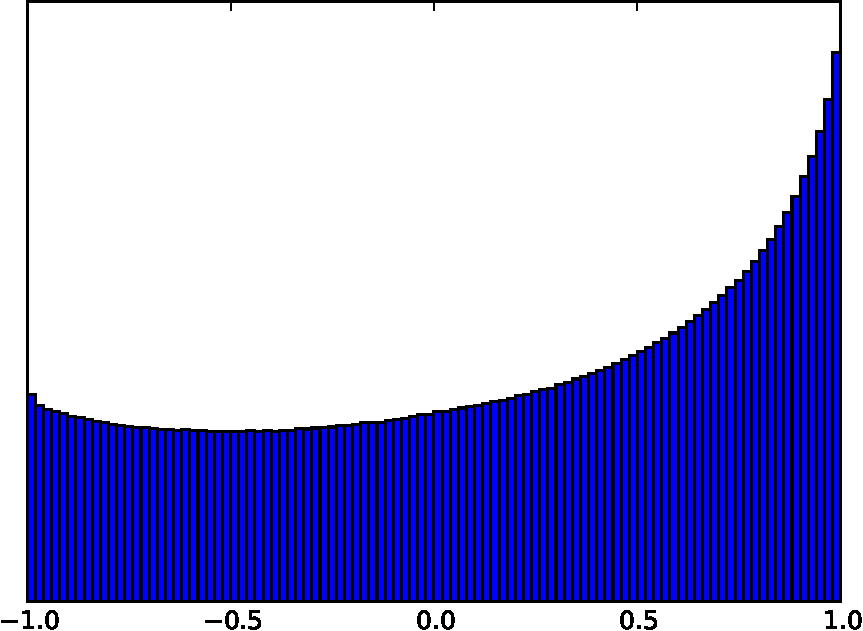
\includegraphics[width=\textwidth]{statistical_normals/images/distributions/inner_product_all-crop}
        \caption{$\cos{\sigma}$ entire image}\label{subfig:singl_img_inner_product_all}
    \end{subfigure} \hfill
    \begin{subfigure}[t]{0.32\textwidth}
        \centering
        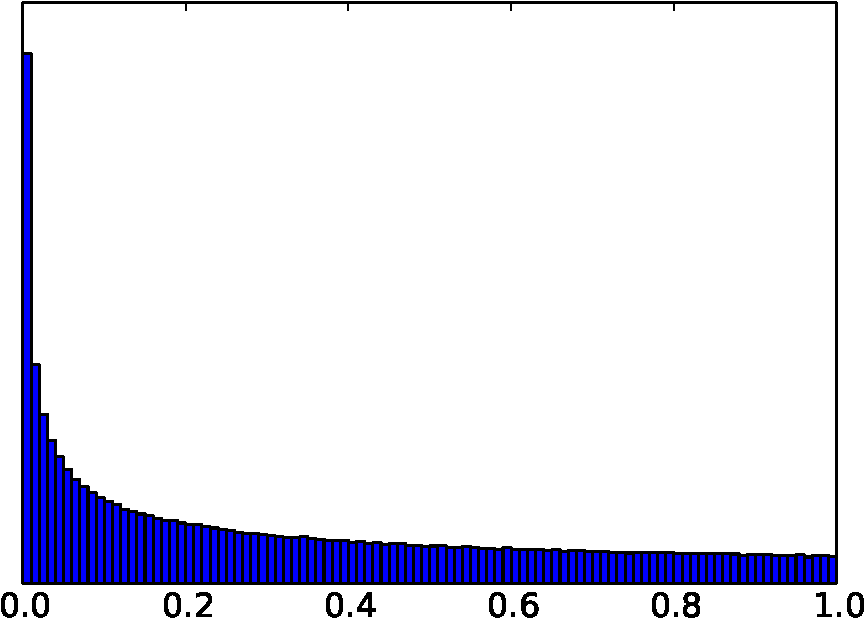
\includegraphics[width=\textwidth]{statistical_normals/images/distributions/inner_product_squared_tumour-crop}
        \caption{$\cos^{2}{\sigma}$ tumour area}\label{subfig:singl_img_inner_product_squared_tumour}
    \end{subfigure}
    \hspace*{\fill}
    \caption{The distributions of $\cos{\sigma}$ and $\cos^2{\sigma}$ averaged
             over 10 subjects from the BraTS simulated images. The images were
             registered using a rigid transformation prior to computation and
             only the tumour areas were sampled. (a) shows the distribution of
             $\cos{\sigma}$ in the simulated tumour region. (b) shows the
             distribution of $\cos{\sigma}$ over the entire image. (c) shows the
             distribution of $\cos^2{\sigma}$ proposed
             in~\cite{haber2006intensity} in the simulated tumour region}
\label{fig:singl_img_inner_product_distributions}
\end{figure*}
%%%%%%%%%%%%%%%%%%%%%%%%%%%%%%%%%%%%%%%%
A more general angular measure between two vectors is the inner product. Unlike
in~\cite{tzimiropoulos2012subspace,tzimiropoulos2011robust} or
\cref{subsubsec:singl_img_cosine_spherical}, the inner
product is a single angle and not the difference between two angles.
Practically, the inner product measures the projection error between two vectors
and is defined as:
%%%%%%%%%%%%%%%%%%%%%%%%%%%%%%%%%%%%%%%%%%%%%%%%%%%%%%%%%%%%%%%%%%%%%%%%%
\begin{equation}\label{eq:singl_img_inner_product}
    \cos{\sigma} = \bb{\tilde{g}}_{1}^{\top} \bb{\tilde{g}}_{2}
\end{equation}
%%%%%%%%%%%%%%%%%%%%%%%%%%%%%%%%%%%%%%%%%%%%%%%%%%%%%%%%%%%%%%%%%%%%%%%%%
This can similarly be performed for 2.5D data by using the surface normals and
thus substituting $\bb{n}$ for $\bb{g}$ in \cref{eq:singl_img_inner_product}.

In~\cite{tzimiropoulos2012subspace,tzimiropoulos2010robust},
the authors reasonably propose that the angle between the
gradients of dissimilar images can take any value in $[0, 2\pi)$ with equal
probability. Similarly, the relationship between the gradient vectors of two
dissimilar 3D images could feasibly be in any direction with equal probability.
Therefore, the distribution of inner products between two unrelated vectors can
take the values $[-1, 1]$ with equal probability. Due to the expected range of
inner product values, we would expect that $\cos{\sigma}$ follows a uniform
distribution, $\cos{\sigma} \sim U(-1, 1)$. Note that this is a different
assumption to that made in~\cite{tzimiropoulos2011robust}, which assumes that the
\textit{azimuth angle itself}, $\Delta \phi$, follows a uniform distribution.
However, it is merely sufficient that the total sum of values from the
dissimilar vectors is zero. Therefore, since $E\{U(-1, 1)\} = 0$, the inner
product of normalised gradients satisfies our definition of being robust to
outliers. In \cref{subfig:singl_img_inner_product_tumour}, we show that this
assumption holds for the simulated tumour data taken from the 
BraTS\footnote{\url{http://www2.imm.dtu.dk/projects/BRATS2012/}} challenge.

When the entire region of the rigidly registered brain images is considered, we
find that the distribution of $\cos{\sigma}$ is clearly a mixture of two
separate models, one for the occluded area and one for the rigidly registered
area. \cref{subfig:singl_img_inner_product_all} shows the distribution of
$\cos{\sigma}$ calculated over the entire image region. In this case, the
distribution of the inner product appears to be a mixture model between a
uniform distribution and a zero mean Laplacian distribution. However, due to the
ambiguity in the inner product in terms of orientation, the angle of the inner
product is only defined in the range $[0, \pi]$ and thus only the positive tail
of the Laplacian appears.

In \cref{subfig:singl_img_inner_product_squared_tumour} we also show the
distribution of the similarity measure proposed by \citet{haber2006intensity}.
In~\cite{haber2006intensity}, the authors propose the inner product as a
similarity measure, which looks very similar to the measure we proposed in
\cref{eq:singl_img_inner_product}. 
However, \citet{haber2006intensity} maximise the square of the
inner product using a least squares Gauss-Newton optimisation. As we have shown,
the inner product is related to the cosine between the vectors.
\citet{haber2006intensity} proposed the inner product squared as
a similarity, which is equivalent to the \textit{square of the cosine}. As we
can see in \cref{subfig:singl_img_inner_product_squared_tumour}, the cosine squared
does not represent a symmetric distribution and therefore is not a robust
similarity measure by our definition.
%%%%%%%%%%%%%%%%%%%%%%%%%%%%%%%%%%%%%%%%%%%%%%%%%%%%%%%%%%%%%%%%%%%%%%%%%%%%%%%%
